\newpage

\section{Pulse Width Modulation (PWM) and Servo Calibration (pulse = f(angle))}

\subsection{Parts List}

\begin{enumerate}[itemsep=-5pt]
\item CPX/CPB
\item USB Cable
\item Laptop
\item a pendulum (can use paper towel roll and some twine)
\item servo
\item Alligator clips (x3)
\end{enumerate}

\subsection{Learning Objectives}
\begin{enumerate}[itemsep=-5pt]
\item Understand what a PWM signal is and how it affects a servo
\item Understand the inner workings of a servo and how to make it move
\item Practice first order regression and calibration techniques
\end{enumerate}

\subsection{Getting Started}

For this lab we are going to learn how to drive a \href{https://www.adafruit.com/product/1143}{servo}. Servos accept what are called PWM signals which are basically square waves of varying frequency. The servo itself has a microprocessor on board that turns a DC motor based on the incoming PWM frequency which is typically called a duty cycle. The DC motor runs through some gear to rotate a shaft. Because of this rotation, you can make a number of things move! Servos are used for all sorts of things, opening doors, deflecting control surfaces on RC aircraft and many more! The neat thing about PWM signals is that they can not only move servos but they can also drive speed controllers to turn 3 phase motors and even change the light intensity of LEDs. Servos typically come in two different color schemes as shown below.
\begin{figure}[H]
  \begin{center}
    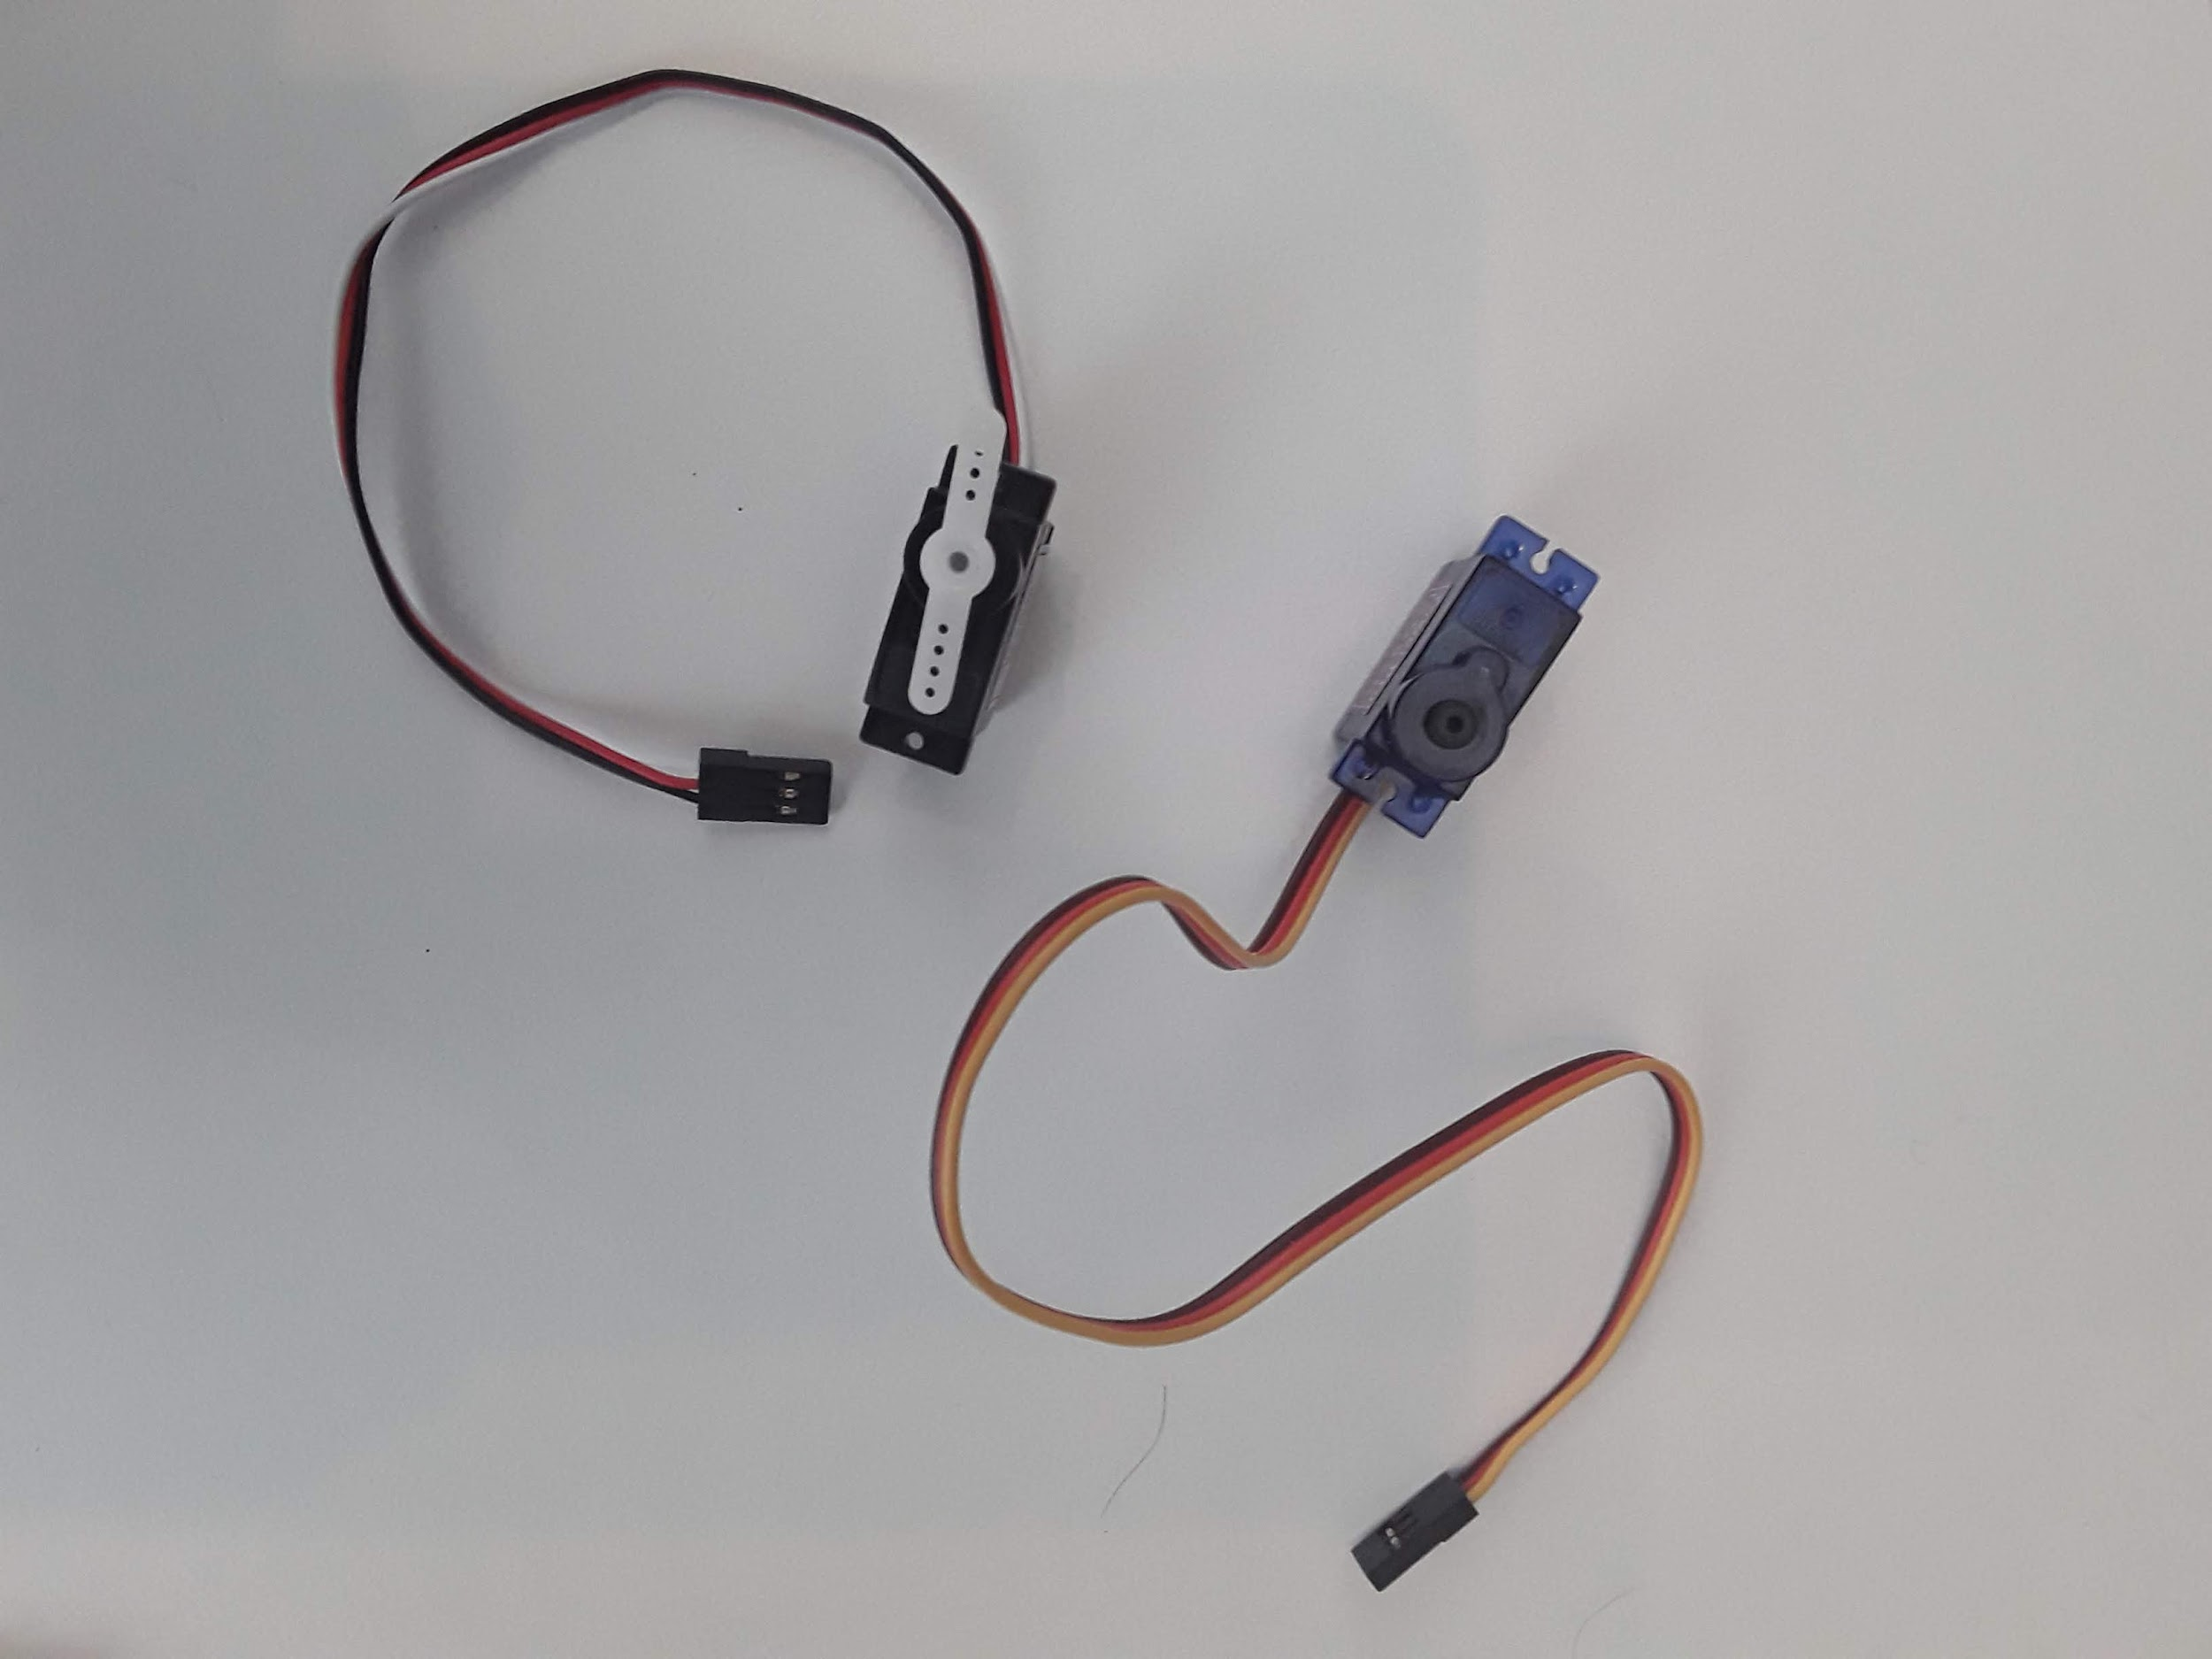
\includegraphics[width=0.8\textwidth]{Figures/servo.jpeg}
  \end{center}
\end{figure}
As you can see, servos have 3 pins - the brown or black wire is GND, the red wire needs to go to a 5V signal so for the CPX it needs to go to the VOUT pin and the yellow or white wire is the signal wire which need to go to an analog port on the CPX that supports PWM signals. Which ones support PWM signals? \href{https://learn.adafruit.com/adafruit-circuit-playground-express/pinouts}{Adafruit Learn} has a great description of which pins support PWM signals but as a quick check you can use the following analog pins: A1, A2, A3, A6 and A7. In my circuit I just picked pin A2 since I’ve been using it so much in the past.
\begin{figure}[H]
  \begin{center}
    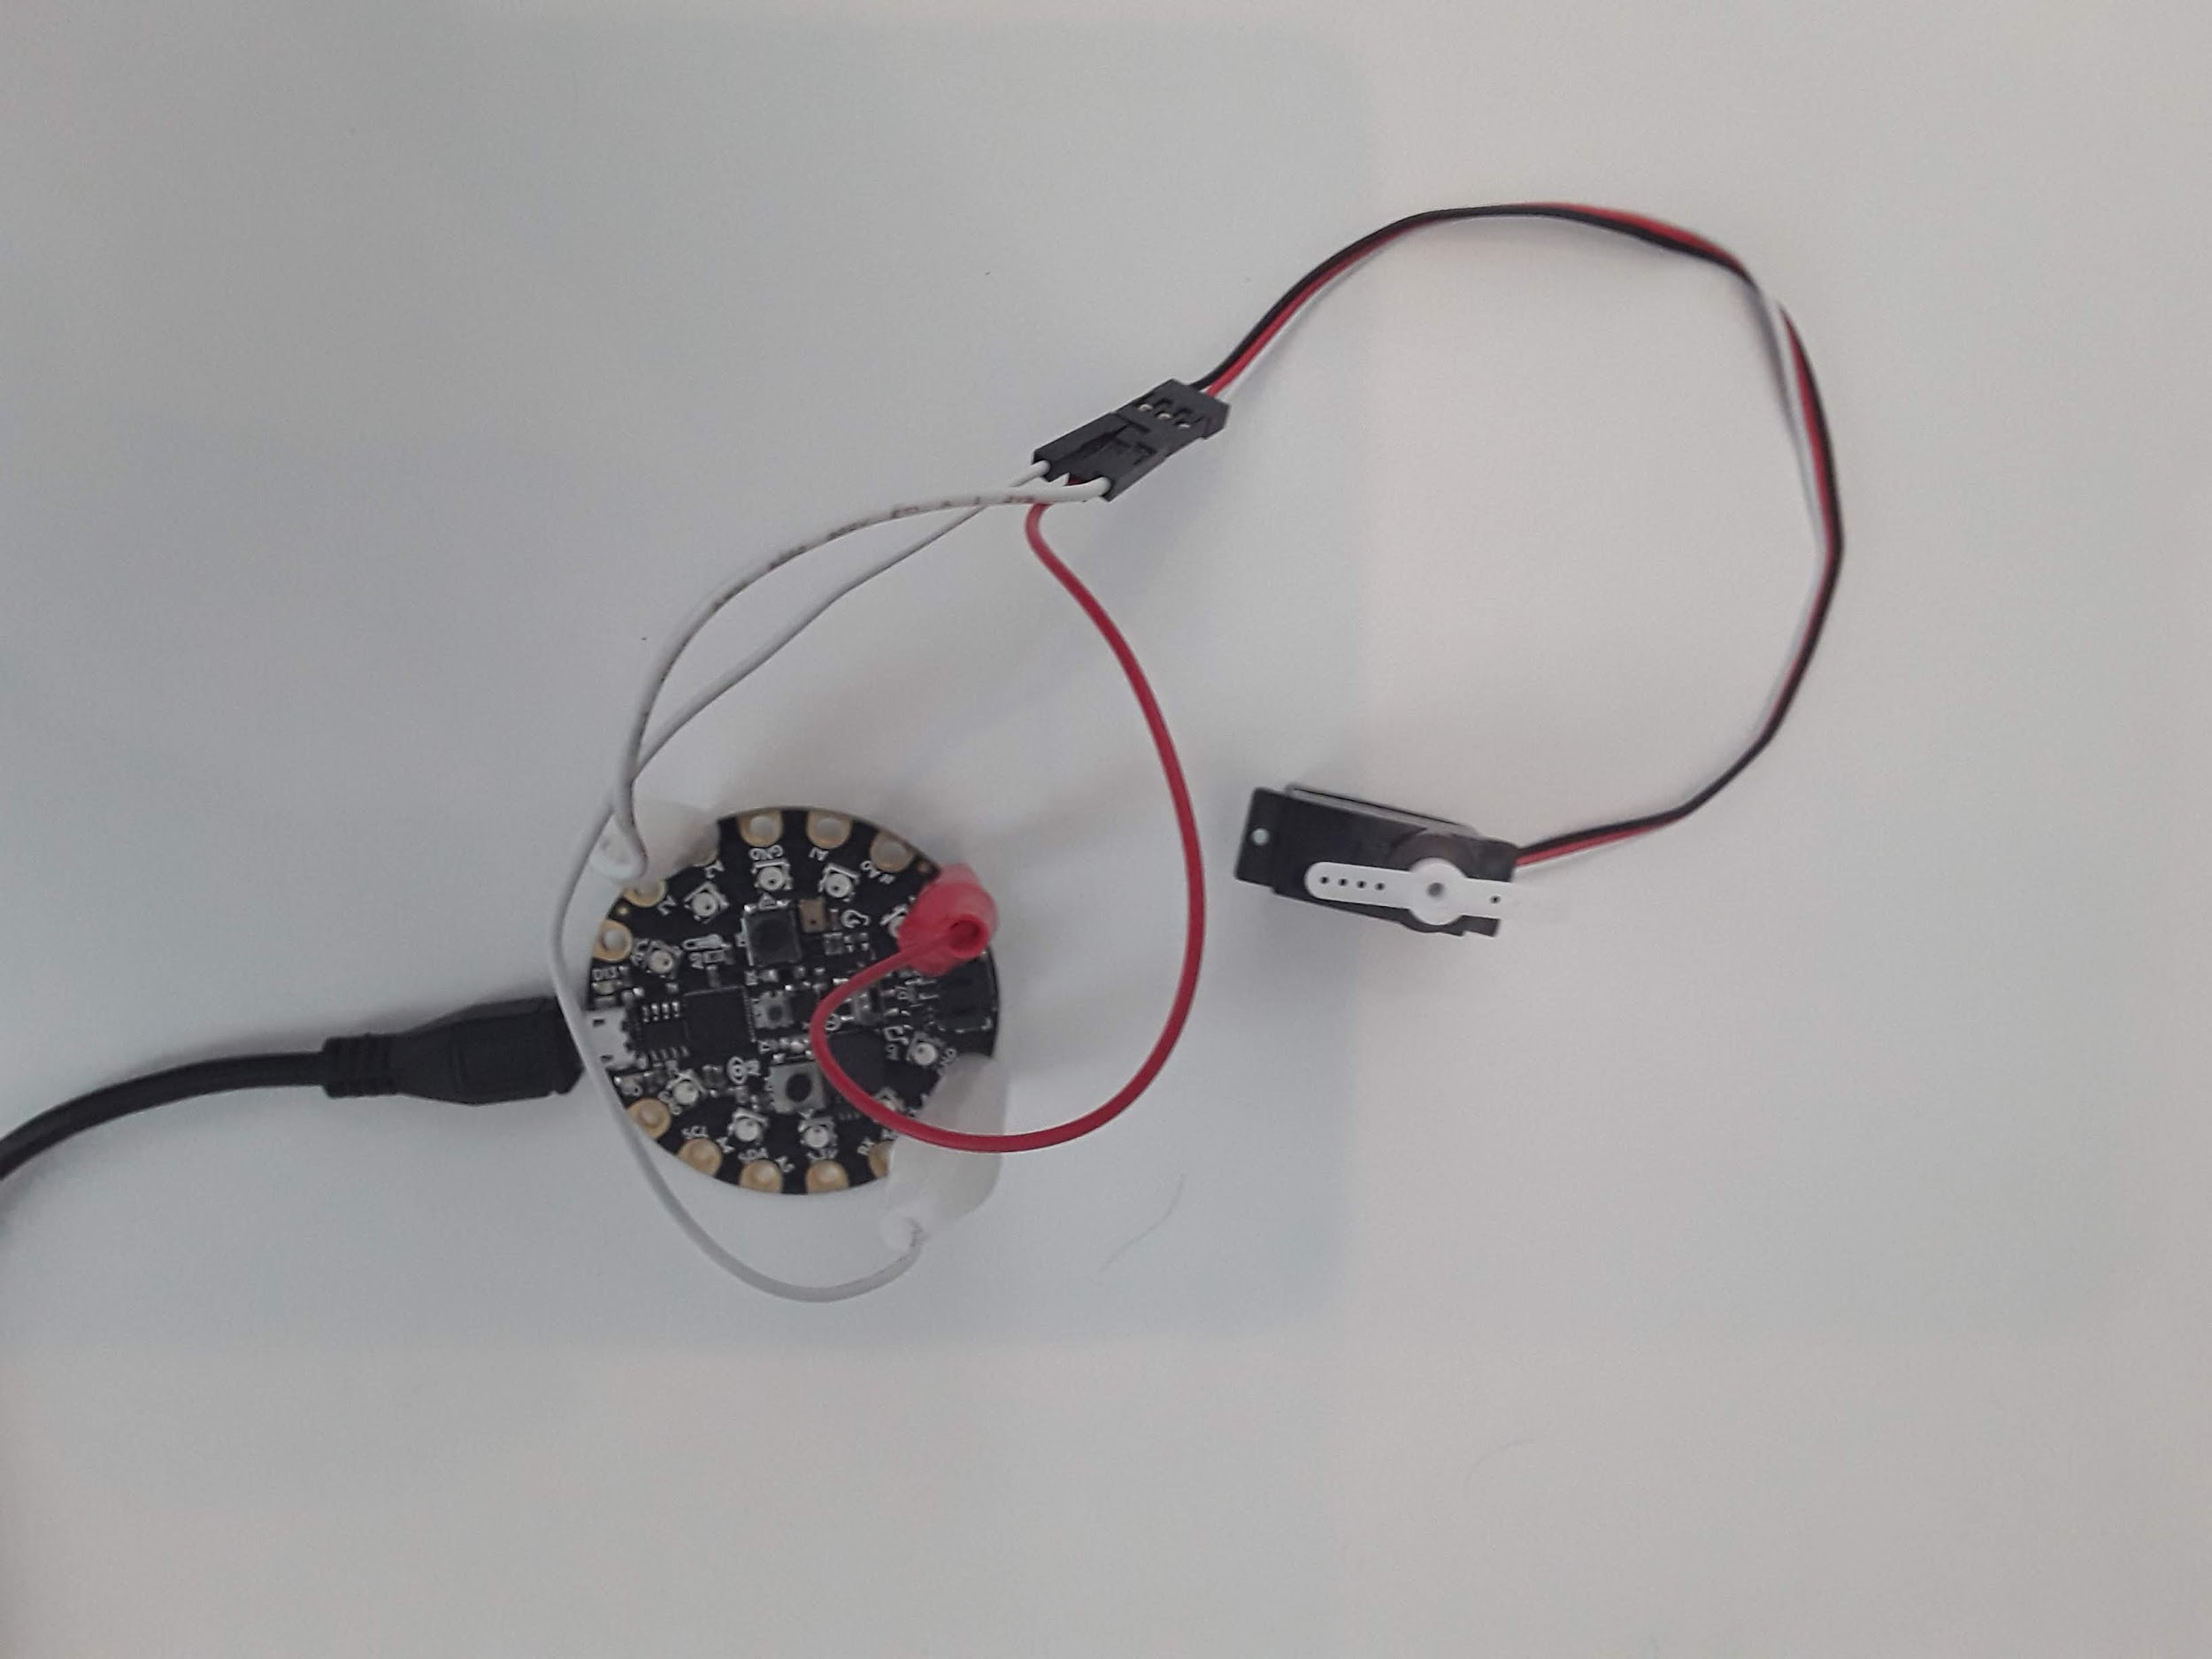
\includegraphics[width=0.8\textwidth]{Figures/servo_circuit.jpeg}
  \end{center}
\end{figure}
{\bf Very important: It is recommended to power a servo through an external power supply instead of the CPX. Servos can draw a lot of current and the CPX although it supports 5V can only provide so much power (P). Remember that P = VI so if P is low it means current is low. If the servo pulls more current than the CPX can provide the CPX will “brown out” which means it will go into a safe-mode setting. If you have the AA power supply you may consider doing that. For small servos you hopefully won’t have any issues.}

    As I said before, a servo takes in a square wave. The square wave has a duty cycle in units of microseconds. If you send a roughly 500 us square wave to a servo it will rotate all the way to the left. If you send a roughly 2500 us signal to the servo, it will turn all the way to the right. The code to send PWM signals has been thoroughly explained in the \href{https://learn.adafruit.com/using-servos-with-circuitpython/overview}{Adafruit Learn system}. I also have a \href{https://github.com/cmontalvo251/Microcontrollers/blob/master/Circuit_Playground/CircuitPython/Servo/servo.py}{simple servo.py script} on Github. In this code as usual the top 3 lines are used to import the necessary modules. The pulseio module is used here to create a servo object on line 6 by connecting to pin A2. Make sure to change the pin to whatever pin you have the signal wire hooked up to. Lines 9-12 create a function that pulse in milliseconds and compute the duty cycle of PWM signal. Lines 16-19 then kick off an infinite while loop where a 800 us signal is sent to the servo and then a 2000 us signal is sent using a for loop which starts on line 16. You’ll see servo command on line 18 which is responsible for sending the microsecond signal to the servo. The function servo\_duty\_cycle converts the pulse in milliseconds to a duty cycle. The value is then passed to the attribute of the servo object servo.duty\_cycle. If you put this code on the CPX and run the code you will hopefully see your servo turning left and right in 1 second intervals. I did this project myself and \href{https://youtu.be/ynlGiPZk5VM}{posted a YouTube video about it}. 

Besides making the servo move back and forth I’d like you to vary the pulses on line 16 {\bf SLOWLY} until the servo can’t move any farther. This line of code is a for loop which loops through the array currently showing [0.8,2.0]. If you change that array to [0.9,1.2,1.5,1.8] the servo will move to a pulse in milliseconds of 0.9, 1.2, 1.5 and then 1.8. The for loop is a great way to loop through multiple commands. Using this array, determine the minimum pulse you can send to the servo and the maximum pulse you can send to the servo. If the servo makes a funny noise it means you sent a signal outside the bounds so try a different signal. Hence the need for moving the pulse signal slowly. If you change the array to just 1 number [0.8] the servo will just move to 1 angle and stay there forever. {\bf NOTE THAT IN CIRCUITPYTHON VERSION 7.0.0 YOU HAVE TO USE THE PWMIO LIBRARY INSTEAD OF THE PULSEIO LIBRARY}.

\begin{figure}[H]
  \begin{center}
    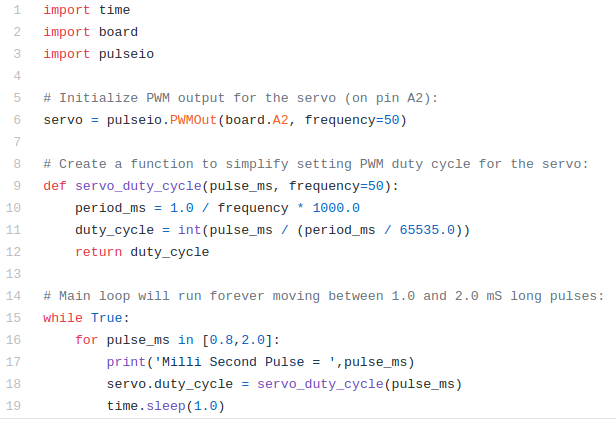
\includegraphics[width=0.8\textwidth]{Figures/servo_code.png}
  \end{center}
\end{figure}
If you notice, sending a pulse signal in microseconds moved the servo to a specific angle. Thing is I would like to be able to move the servo to a specific angle rather than having to just guess and check like we did in the last lab. So what we’re going to do is start at the minimum pulse signal you computed in the last project and then change the servo pulse in equal increments until we reach the maximum servo pulse signal. When I did this lab I found that 0.6 ms was just about the smallest I could get the servo to move. We’re going to call this 0 degrees. My maximum pulse signal ended up being about 2.4 ms. So I want you to test 10 different points between your specific maximum and minimum value which will hopefully be different for all of you. Everytime you test a pulse I want to measure the angle the servo makes with the minimum value being 0 degrees. Create a table of data with two columns. In the first column put pulse in milliseconds and in the second column put angle of servo in degrees. Use a protractor to measure the angle. \href{https://www.youtube.com/watch?v=XSLzcwTOsWk}{If you don’t have a protractor make one} or you can download a picture and hold your servo up to the screen. I did this project with just 3 data points and here are my data points. Again you need to have around 10 data points
\begin{table}[H]
\begin{center}
\begin{tabular}{|c|c|}
\hline
Pulse (ms) & Angle (Degrees) \\
\hline
0.6 & 0 \\
\hline
1.5 & 90 \\
\hline
2.4 & 180 \\
\hline
\end{tabular}
\end{center}
\end{table}

\subsection{Assignment}

Upload a PDF with all of the photos and text below included. My recommendation is for you to create a Word document and insert all the photos and text into the document. Then export the Word document to a PDF. For videos I suggest uploading the videos to Google Drive, turn on link sharing and include a link in your PDF.
\subsubsection{Part 1}
\begin{enumerate}[itemsep=-5pt]
\item Send a video of your servo moving back and forth (make sure your face is in the video and make sure you introduce yourself) - 50\%
\item Experimentally determine the minimum and maximum values of the servo and report the 2 PWM signals in milliSeconds. Give at least 2 decimal points in your calculation - 50\%
\end{enumerate}
\subsubsection{Part 2}
\begin{enumerate}[itemsep=-5pt]
\item Submit a video of you explaining how you took data (make sure you are in the video and you introduce yourself) - 25\%
\item Include a Figure of your your data plotted in Python with your trend line on top - 25\%
\item Submit your regression equation as I did above - 25\%
\item Submit a video of your servo moving through 0,45,90,135 using the output from your regression equation. -  25\% 
\end{enumerate}